\chapter{Modellazione degli ambienti}
\label{sec:4_modellazione}

In questo capitolo viene descritta la modellazione degli ambienti proposti per la distribuzione del carico all'interno di un sistema edge-FaaS. Sono stati modellati tre ambienti multi-agente, di complessità incrementale, insieme alle dinamiche in cui le policy operano. Diverse ipotesi semplificatrici sono state introdotte rispetto allo scenario reale per investigare se il Reinforcement Learning può essere una valida soluzione per la distribuzione del carico, con l'obiettivo finale di progettare un ambiente reale multi-agente adatto per la piattaforma DFaaS.

Come introdotto nella \Cref{sec:2_mdp}, un ambiente MARL è caratterizzato da uno spazio delle osservazioni e delle azioni per ogni agente, una funzione di ricompensa per agente e uno stato interno (globale o locale) dell'ambiente che contiene informazioni sul sistema simulato.

Nelle seguenti sezioni sono dettagliate le singole proprietà degli ambienti modellati.

\section{Elementi del sistema}
\label{sec:4_modellazione_elementi}

Data la moltitudine di elementi che compongono il problema affrontato, in questa sezione sono raccolti in un unico posto tutte le variabili che definiscono l'ambiente con una definizione concisa.

Due insiemi importanti sono l'insieme degli agenti $\mathcal{N}$ e l'insieme dei passi $T$, entrambi finiti in $\mathbb{N}^0$. Ogni variabile fa riferimento a un agente $n \in \mathcal{N}$ al $t$-esimo passo\footnote{Gli indici dell'agente o del passo sono omessi a meno di ambiguità.} ($t \in T$):

\begin{itemize}
    \item Richieste in input $R^\textnormal{IN}$: rappresenta il numero di richieste in ingresso che l'agente che deve distribuire.

    \item Capacità della coda $q^\textnormal{MAX}$: rappresenta il numero di slot disponibili che si possono utilizzare per processare localmente le richieste.

    \item Capacità residua della coda $q^\textnormal{FREE}$: rappresenta il numero di slot disponibili a seguito dell'allocazione delle richieste da processare localmente.

    \item Capacità di inoltro $F$: rappresenta il numero di richieste che un agente può inoltrare ad altri agenti.

    \item Eccesso di processamento locale $e^\textnormal{L}$: rappresenta il numero di richieste che l'agente ha tentato di processare localmente ma che eccedono la capacità della coda, e che pertanto sono considerate rifiutate.

    \item Eccesso di rifiuto $e^\textnormal{R}$: rappresenta il numero di richieste rifiutate che potevano essere processate localmente oppure inoltrate senza essere rifiutate.

    \item Eccesso di inoltro $e^\textnormal{FW}$: rappresenta il numero di richieste inoltrate in eccesso, cioè richieste che sono state inoltrate ma che potevano essere processate localmente.

    \item Richieste inoltrate ma rifiutate $e^\textnormal{FR}$: rappresenta il numero di richieste inoltrate da un agente che sono state rifiutate dagli altri agenti. È anche indicato come $s^\textnormal{FR}$ se la variabile fa riferimento all'osservazione.
\end{itemize}

\section{Definizione degli ambienti}
\label{sec:4_environments}

I tre ambienti modellati differiscono per la capacità degli agenti di inoltrare o meno le richieste in ingresso agli altri agenti. Di complessità incrementale, ad alto livello sono così definiti:

\begin{itemize}
    \item \textbf{Ambiente simmetrico senza inoltro}: gli agenti sono completamente indipendenti l'uno dall'altro e possono soltanto processare localmente o rifiutare le richieste in arrivo. Etichettato come ``BASE'' di seguito.

    \item \textbf{Ambiente asimmetrico}: gli agenti sono divisi in due gruppi disgiunti, uno in grado di inoltrare le richieste agli altri nodi e uno che può soltanto processare le richieste localmente o rifiutarle. Etichettato come ``ASYM'' di seguito.

    \item \textbf{Ambiente simmetrico con inoltro}: ogni agente può processare localmente, inoltrare agli altri agenti o rifiutare le richieste in ingresso. Etichettato come ``SYM'' di seguito.
\end{itemize}

I tre ambienti sono raffigurati in \Cref{fig:4_environments} in una configurazione a due agenti.

\begin{figure}
    \centering

    \begin{subfigure}{.6\textwidth}
        \centering
        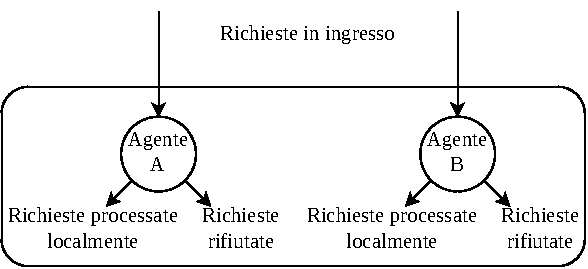
\includegraphics[width=\linewidth]{assets/4/1_sym_no_fw.pdf}
        \caption{Simmetrico senza inoltro}
    \end{subfigure}

    \begin{subfigure}{.6\textwidth}
        \centering
        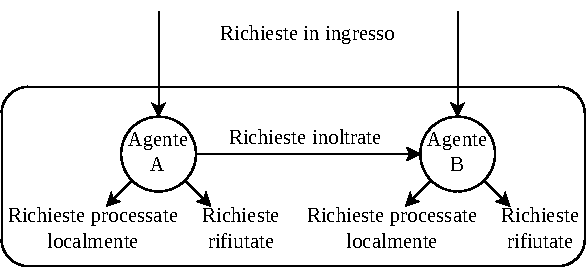
\includegraphics[width=\linewidth]{assets/4/2_asym.pdf}
        \caption{Asimmetrico}
    \end{subfigure}

    \begin{subfigure}{.6\textwidth}
        \centering
        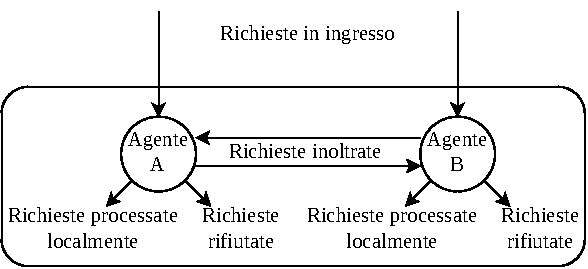
\includegraphics[width=\linewidth]{assets/4/3_sym_fw.pdf}
        \caption{Simmetrico con inoltro}
    \end{subfigure}
    
    \caption{I tre ambienti progettati con due agenti ciascuno.}
    \label{fig:4_environments}
\end{figure}

In ogni passo, ogni agente dell'ambiente agisce in un determinato spazio delle azioni, guidato dalle informazioni contenute nello spazio delle osservazioni. In risposta all'azione, l'ambiente restituisce agli agenti una ricompensa, calcolata dalla funzione di ricompensa. Le seguenti tre sottosezioni definiscono in modo formale i tre elementi.

\subsection{Spazio delle azioni}

La decisione consiste nel numero di richieste da processare localmente, inoltrare e rifiutare. Formalmente, si considera uno spazio di azioni continuo $\mathcal{A}$ i cui elementi sono delle tuple $(p^\textnormal{L}, p^\textnormal{F}, p^\textnormal{R})$, ogni $p^x$ è la percentuale di richieste da processare, inoltrare e rifiutare. Le percentuali fanno riferimento al numero di richieste in ingresso, informazione contenuta nello spazio delle osservazioni.

Per gli ambienti simmetrici senza inoltro e asimmetrici, lo spazio si riduce a tuple $(p^\textnormal{L}, p^\textnormal{R})$ per gli agenti che non possono inoltrare le richieste.

\subsubsection{Distribuzione di Dirichlet}

Un vincolo importante per lo spazio delle azioni è che un'azione $a \in \mathcal{A}$ soddisfi il vincolo

\begin{equation}\label{eq:4_simplex_condition}
    p^\textnormal{L} + p^\textnormal{F} + p^\textnormal{R} = 1.
\end{equation}

Analogamente, le azioni degli agenti che non possono inoltrare devono soddisfare $p^\textnormal{L} + p^\textnormal{R} = 1$. Il motivo è che, come introdotto sopra, le azioni rappresentano la percentuale (o proporzione) di richieste da distribuire nei modi definiti, pertanto tutte e sole le richieste devono essere distribuite.

\paragraph{Il simplesso.} Il vincolo in \Cref{eq:4_simplex_condition} può essere rappresentato con un \mbox{2-simplesso}, cioè un triangolo equilatero con vertici $(1, 0, 0), (0, 1, 0), (0, 0, 1) \in \mathbb{R}^3$. Ciascun asse rappresenta una delle tre azioni possibili. Ogni punto all'interno o sulla superficie del triangolo soddisfa il vincolo in \Cref{eq:4_simplex_condition}. La \Cref{fig:4_simplex} mostra il 2-simplesso con esempi di punti presi all'interno dello spazio.

Il simplesso definisce dei limiti precisi in cui l'agente può prendere le decisioni, garantendo che la somma delle azioni copra l'intero insieme delle richieste in ingresso. I vertici del simplesso indicano delle azioni ``estreme'': con $(1, 0, 0)$ l'agente elabora tutte le richieste localmente, con $(0, 1, 0)$ l'agente inoltra tutte le richieste e con $(0, 0, 1)$ l'agente rifiuta tutte le richieste.

\paragraph{La distribuzione.} Gli algoritmi di RL progettati per spazi d'azione continui, come in questo problema, non possono generare una policy imparando la probabilità di selezionare un'azione specifica nello stato attuale, come viene solitamente fatto quando $\mathcal{A}$ è un insieme finito (e non eccessivamente grande). Invece, gli agenti imparano ad approssimare, dallo stato attuale, i parametri di una distribuzione di probabilità sulle azioni, e l'azione scelta viene estratta da questa distribuzione. Per questo motivo è stata scelta la distribuzione di probabilità di Dirichlet, rispetto alle distribuzioni Gaussiana e Gaussiana-softmax: la prima, tipicamente adottata come distribuzione predefinita nell'algoritmo PPO, non garantisce che le azioni soddisfano il vincolo in \Cref{eq:4_simplex_condition}, mentre la seconda introduce un bias per via della normalizzazione e una maggiore varianza durante l'addestramento, oltre a una convergenza più lenta rispetto a Dirichlet \cite{Tian2022}.

\paragraph{Parametri della distribuzione.} Nel problema specifico, la distribuzione è parametrizzata dal numero di categorie $K$ e da un vettore di concentrazione $\boldsymbol{\alpha} = (\alpha_1, ..., \alpha_K)$. Ogni elemento $\alpha_i$ è un reale positivo e specifica la forma della distribuzione per la singola dimensione: se il valore di $\alpha_i$ è più alto degli altri, i valori estratti dalla distribuzione tendono a preferire la $i$-esima categoria. 

Nel problema specifico, $K = 3$ rimane costante poiché le azioni sono tre, mentre gli agenti imparano il vettore di concentrazione. Lo stesso vale per gli agenti che non possono inoltrare, in cui però $K = 2$.

\begin{figure}
    \centering

    \begin{subfigure}{.45\textwidth}
        \centering
        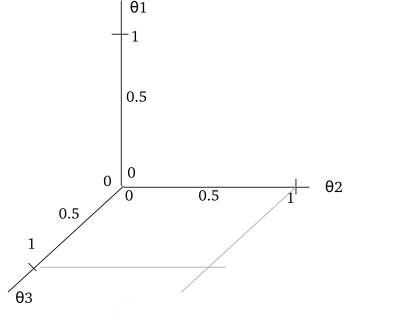
\includegraphics[width=\linewidth]{assets/4/simplex_1.png}
        \caption{}
        \label{fig:4_simplex_1}
    \end{subfigure}%
    \begin{subfigure}{.45\textwidth}
        \centering
        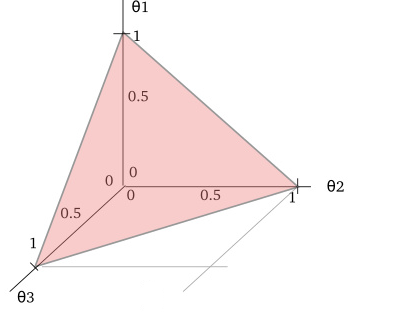
\includegraphics[width=\linewidth]{assets/4/simplex_2.png}
        \caption{}
        \label{fig:4_simplex_2}
    \end{subfigure}

    \begin{subfigure}{.45\textwidth}
        \centering
        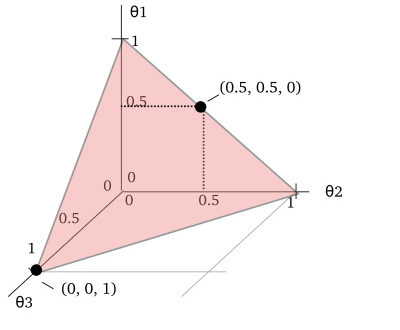
\includegraphics[width=\linewidth]{assets/4/simplex_3.png}
        \caption{}
        \label{fig:4_simplex_3}
    \end{subfigure}%
    \begin{subfigure}{.45\textwidth}
        \centering
        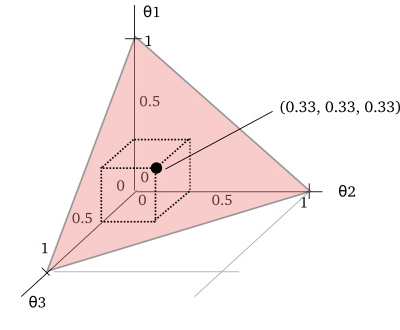
\includegraphics[width=\linewidth]{assets/4/simplex_4.png}
        \caption{}
        \label{fig:4_simplex_4}
    \end{subfigure}

    \begin{subfigure}{.9\textwidth}
        \centering
        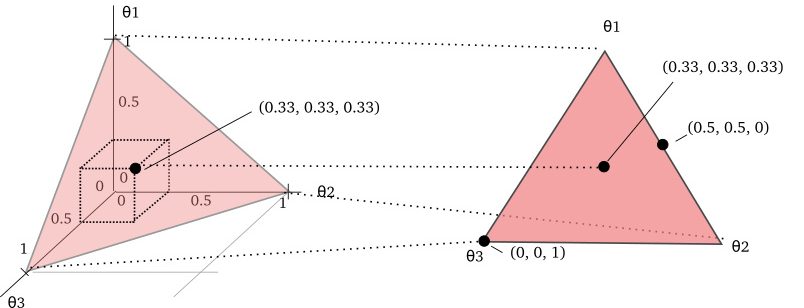
\includegraphics[width=\linewidth]{assets/4/simplex_5.png}
        \caption{}
        \label{fig:4_simplex_5}
    \end{subfigure}

    \caption[Esempio di 2-simplesso]{L'esempio mostra lo spazio tridimensionale con $\theta_{1, 2, 3}$ come coordinate, ogni coordinata può assumere valori nell'intervallo $[0, 1] \in \mathbb{R}$ (\Cref{fig:4_simplex_1}). \Cref{fig:4_simplex_2} mostra il 2-simplesso sullo spazio. \Cref{fig:4_simplex_3,fig:4_simplex_4} mostrano tre esempi di punti sul simplesso per cui vale il vincolo $\theta_1 + \theta_2 + \theta_3 = 1$. Infine \Cref{fig:4_simplex_5} mostra la proiezione del simplesso su due dimensioni con i punti mostrati in precedenza. Fonte: \url{https://stats.stackexchange.com/a/296779}}
    \label{fig:4_simplex}
\end{figure}

\begin{figure}
    \centering
    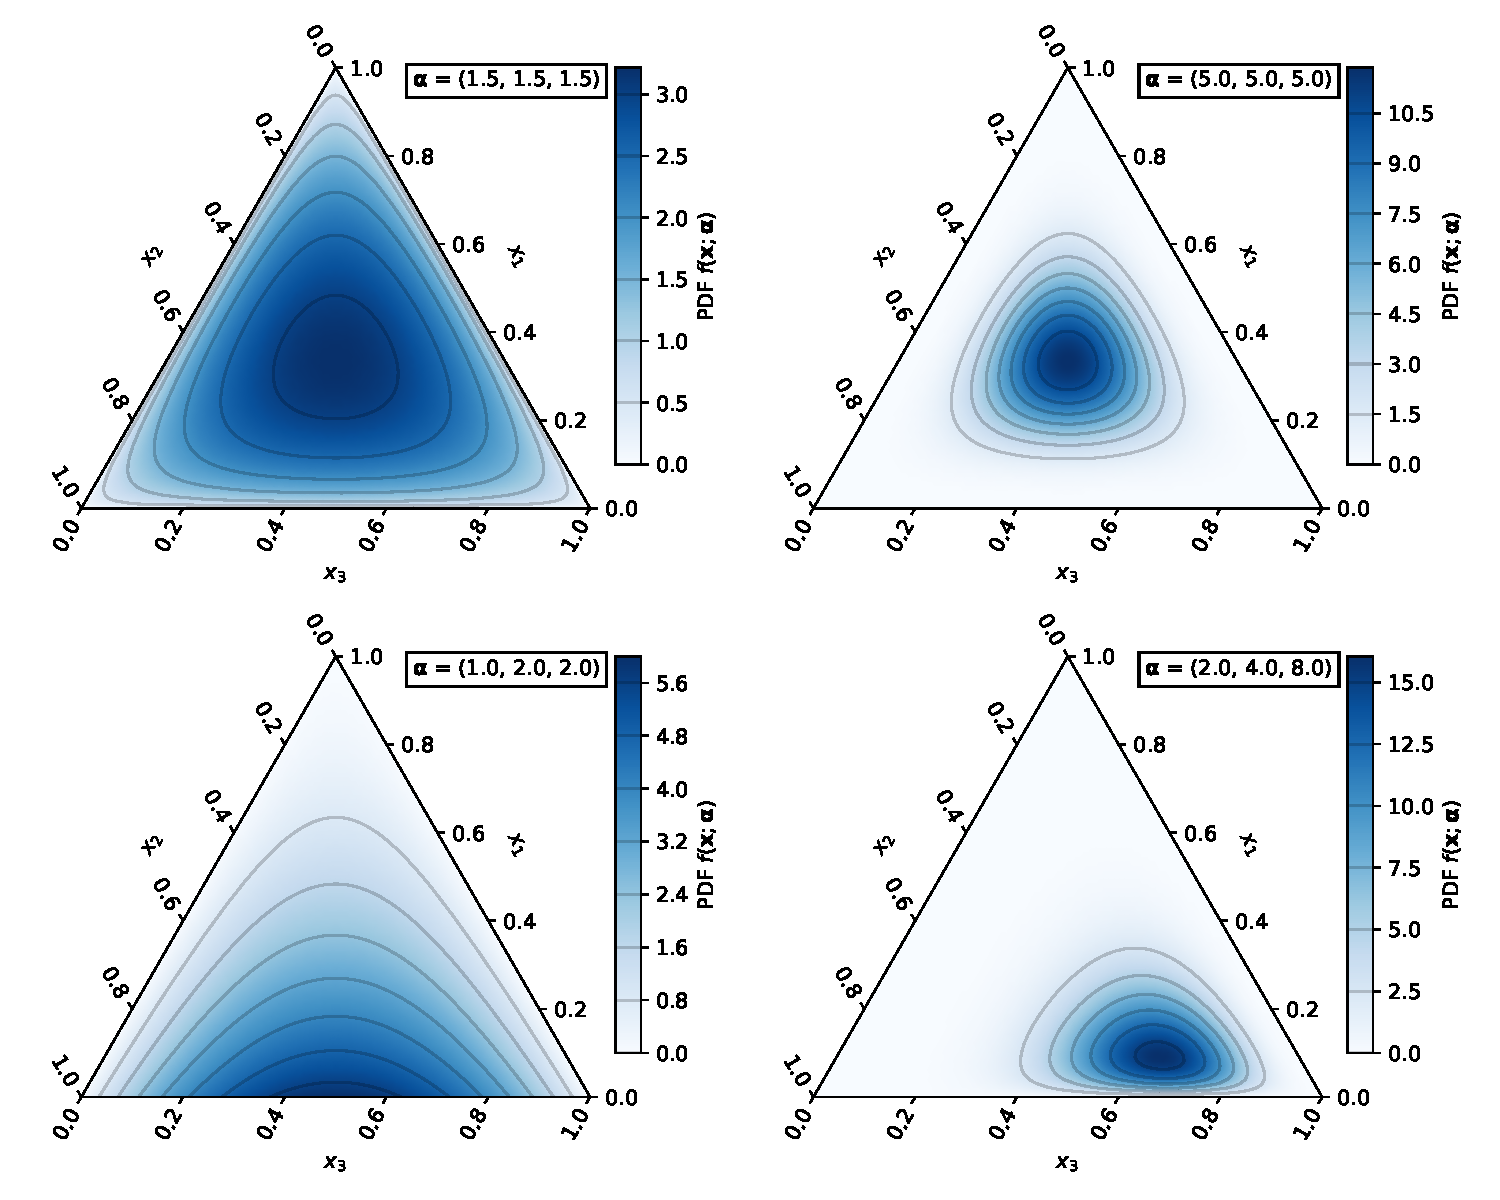
\includegraphics[width=\linewidth]{assets/4/dirichlet_concentration.pdf}
    \caption[Esempio di variazione dei parametri di concentrazione per Dirichlet]{Esempio di funzioni di densità di probabilità per le distribuzioni Dirichlet sul 2-simplesso al variare dei parametri di concentrazione. I valori delle funzioni sono mostrati dal colore con le linee di contorno che corrispondono al valore indicato nelle barre laterali. Fonte: Nerebur, CC BY-SA, Wikipedia Commons.}
    \label{fig:4_dirichlet_concentration}
\end{figure}

\subsection{Spazio delle osservazioni}

Ogni agente osserva uno stato $s \in \mathcal{S}$ definito dalla tupla $s = (R^\textnormal{IN}, q^\textnormal{FREE}, s^\textnormal{F}, s^\textnormal{FR})$: $R^\textnormal{IN}$ è il numero di richieste in ingresso, $q^\textnormal{FREE}$ è il numero di slot disponibili della coda per processare localmente le richieste, $s^\textnormal{F}$ sono il numero richieste inoltrate al passo precedente e $s^\textnormal{FR}$ sono le richieste inoltrate ma rifiutate nel passo precedente. Valgono sempre le seguenti condizioni: $R^\textnormal{IN} \ge 0$ e $s^\textnormal{FR} \le s^\textnormal{F}$.

Per l'ambiente asimmetrico e simmetrico senza inoltro, alcuni agenti non possono inoltrare le richieste e lo spazio si riduce a una tupla $s = (R^\textnormal{IN}, q^\textnormal{FREE})$.

\paragraph{Coda locale.} La gestione del carico all'interno di un singolo nodo avviene con una dinamica semplificata: la coda per l'elaborazione locale si svuota completamente a ogni passo, e diamo priorità alle richieste locali prima di gestire le richieste inoltrate ricevute da altri nodi. Quest'ultimo comportamento è stato scelto per essere più simile a come funziona DFaaS. Per questo motivo $q^\textnormal{FREE}$ nello stato coincide con $q^\textnormal{FREE}$. 

\subsection{Funzioni di ricompensa}
\label{sec:4_funzione_ricompensa}

La funzione di ricompensa è l'elemento essenziale per guidare gli agenti nel processo di apprendimento della strategia ottimale per distribuire le richieste in ingresso. Sono state definite due distinte funzioni di ricompensa una per gli agenti che non possono inoltrare le richieste e una per gli agenti che possono inoltrare. L'obiettivo comune di entrambe, ad alto livello, è di incentivare l'elaborazione locale delle richieste entro i limiti consentiti dalla capacità residua della coda, per poi inoltrare le richieste in eccesso che possono essere gestite dai nodi vicini, e infine rifiutare le richieste che non è possibile processare o inoltrare.

Per comodità, nelle funzioni di ricompensa non si utilizzano i valori percentuali $(p^\textnormal{L}, p^\textnormal{F}, p^\textnormal{R})$ che corrispondono direttamente all'azione scelta dall'agente, ma valori assoluti, definiti sulla base del carico in ingresso come $r^\textnormal{L} = R^\textnormal{IN} p^\textnormal{L}$, $r^\textnormal{F} = R^\textnormal{IN} p^\textnormal{F}$ e $r^\textnormal{R} = R^\textnormal{IN} p^\textnormal{R}$, per cui $r^\textnormal{L} + r^\textnormal{F} + r^\textnormal{R} = R^\textnormal{IN}$.

\subsubsection{Funzione senza inoltro}
\label{sec:4_reward_no_fw}

La funzione di ricompensa per l'agente in grado solo di processare localmente e rifiutare è definita come:

\begin{equation}
    \mathcal{R}: \mathbb{N}^0 \times \mathbb{N}^0 \times \mathbb{N}^0 \times \mathbb{N}^0 \times \mathbb{N}^0 \longrightarrow [0, 1], \quad 
    r_t = \mathcal{R}(r^\textnormal{L}, r^\textnormal{F}, e^\textnormal{R}, q^\textnormal{FREE}, q^\textnormal{MAX})
\end{equation}

in cui tutte le variabili, a eccezione di $q^\textnormal{MAX}$ che è costante, fanno riferimento a uno specifico agente per il $t$-esimo passo, ottenendo la ricompensa $r_t$.

La variabile $r^\textnormal{L}$ conteggia le richieste che l'agente vuole processare localmente. Tale numero può eccedere il numero di slot disponibili nella coda, perciò l'effettivo numero di richieste processate localmente è $r^\textnormal{L} - e^\textnormal{L}$ e che $e^\textnormal{L} \le r^\textnormal{L}$ è sempre soddisfatta.

La definizione segue $\mathcal{R}(s_t, a_t, s_{t+1})$ introdotta in \Cref{sec:2_reward_function_def} per un processo decisionale di Markov, poiché le variabili sopracitate sono sufficienti per racchiudere l'azione dell'agente, lo stato attuale e successivo dell'ambiente. Infatti dall'azione in valori assoluti si può ricavare il numero di richieste totali, mentre per la coda, poiché si svuota a ogni passo, è sufficiente conoscere lo stato ($q^\textnormal{FREE}$) a seguito della distribuzione delle richieste.

La funzione è composta da quattro casi:

\begin{enumerate}
    \item Se $R^\textnormal{IN} = 0$: caso base in cui la ricompensa è $r_t = 1$, in assenza di richieste da distribuire\footnote{Poiché $r^\textnormal{L}$ e $r^\textnormal{R}$ sono valori assoluti, si può ottenere $R^\textnormal{IN} = r^\textnormal{L} + r^\textnormal{R}$.}.

    \item Se $e^\textnormal{L} > 0$, l'agente ha cercato di processare localmente più richieste della capacità della coda. Più è alto il valore e si riduce la ricompensa, mostrata in \Cref{fig:4_reward_asym_no_fw_only_local}, per cui

    \begin{equation}
        r_t = 1 - \frac{e^\textnormal{L}}{r^\textnormal{L}}.
    \end{equation}

    \item Se $q^\textnormal{FREE} > r^\textnormal{R}$, la capacità residua della coda sarebbe stata sufficiente per processare tutte le richieste che l'agente ha scelto di rifiutare. Più è alta questo rapporto e più viene penalizzata la ricompensa, mostrata in \Cref{fig:4_reward_asym_no_fw_total_reject}, per cui:

    \begin{equation}
        r_t = 1 - \frac{r^\textnormal{R}}{R^\textnormal{IN}}.
    \end{equation}

    \item Se $q^\textnormal{FREE} \le r^\textnormal{R}$, invece ,alcune richieste potevano essere processate localmente, mentre le restanti sono state correttamente rifiutate. Solo le prime vengono penalizzate, come mostrato sempre \Cref{fig:4_reward_asym_no_fw_total_reject}, per cui:

    \begin{equation}
        r_t = 1 - \frac{q^\textnormal{FREE}}{R^\textnormal{IN}}.
    \end{equation}
\end{enumerate}

I quattro casi costituiscono la funzione completa:

\begin{equation}
    \mathcal{R}(\cdot) = \begin{dcases}
        1 & R^\textnormal{IN} = 0 \\
        1 - \frac{e^\textnormal{L}}{r^\textnormal{L}} & e^\textnormal{L} > 0 \\
        1 - \frac{r^\textnormal{R}}{R^\textnormal{IN}} & q^\textnormal{FREE} > r^\textnormal{R} \\
        1 - \frac{q^\textnormal{FREE}}{R^\textnormal{IN}} & q^\textnormal{FREE} \le r^\textnormal{R}
    \end{dcases}
\end{equation}

\begin{figure}
    \centering

    \begin{subfigure}{.7\textwidth}
        \centering
        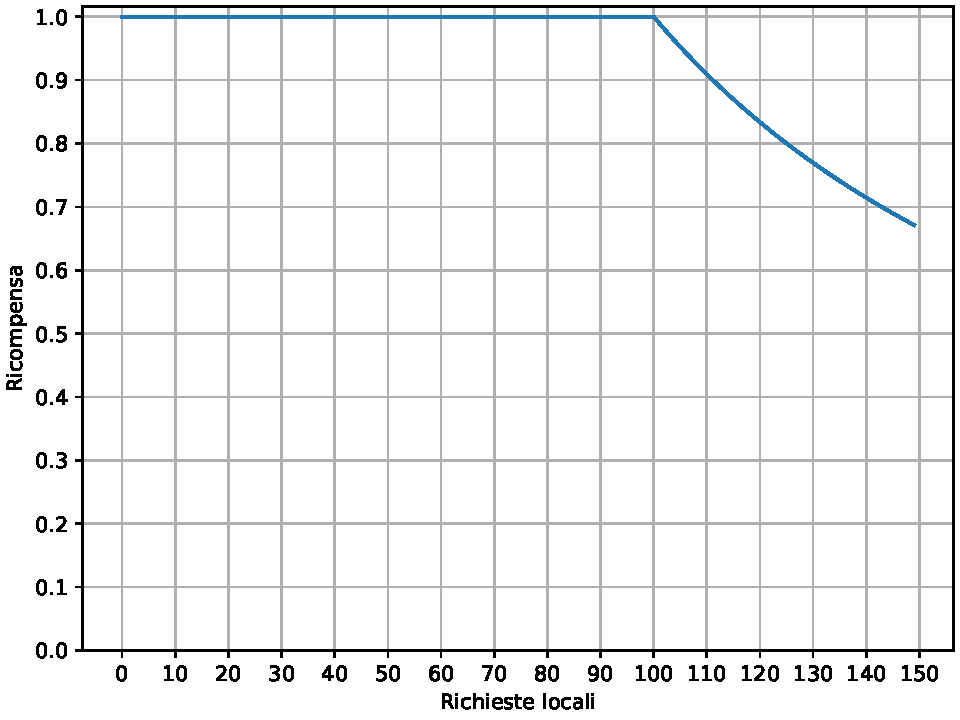
\includegraphics[width=\linewidth]{assets/4/reward_asym_no_forward_local_reqs.pdf}
        \caption{Ricompensa al variare delle richieste processate localmente ($r^\textnormal{R} = 0$).}
        \label{fig:4_reward_asym_no_fw_only_local}
    \end{subfigure}

    \begin{subfigure}{.7\textwidth}
        \centering
        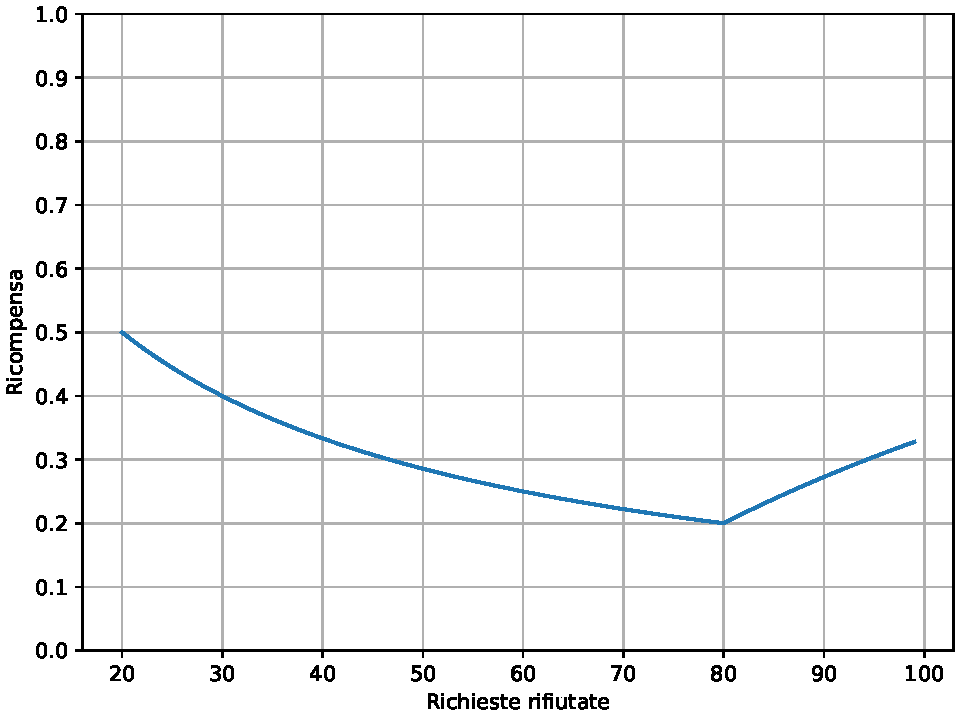
\includegraphics[width=\linewidth]{assets/4/reward_asym_no_forward_total_reject.pdf}
        \caption{Ricompensa al variare delle richieste rifiutate (${r^\textnormal{L} = 20}$). Per $r^\textnormal{R} \le 80$, avendo disponibilità di slot in coda, l'agente avrebbe dovuto processare tutte le richieste localmente. Per $r^\textnormal{R} > 80$, una porzione delle richieste sono inevitabilmente da rifiutare.}
        \label{fig:4_reward_asym_no_fw_total_reject}
    \end{subfigure}
    
    \caption[Esempi di ricompense per la funzione senza inoltro]{Esempi di ricompense per la funzione senza inoltro considerando $q^\textnormal{MAX} = 100$.}
    \label{fig:4_reward_asym_no_fw}
\end{figure}

\subsubsection{Funzione con inoltro}

La funzione di ricompensa per l'agente che è in grado di inoltrare è definita su

\begin{equation}
    \begin{gathered}
        \mathcal{R}^\textnormal{FW}: \mathbb{N}^0 \times \mathbb{N}^0 \times \mathbb{N}^0 \times \mathbb{N}^0 \times \mathbb{N}^0 \times \mathbb{N}^0 \times \mathbb{N}^0 \longrightarrow [0, 1], \\ r_t = \mathcal{R}^\textnormal{FW}(r^\textnormal{L}, r^\textnormal{F}, r^\textnormal{R}, e^\textnormal{L}, e^\textnormal{FR}, q^\textnormal{FREE}, q^\textnormal{MAX}),
    \end{gathered}
\end{equation}

in cui, come per la funzione precedente, tutte le variabili, a eccezione di $q^\textnormal{MAX}$, fanno riferimento a uno specifico agente per il $t$-esimo passo, ottenendo la ricompensa $r_t$.

Per $r^\textnormal{F}$, vale la stessa osservazione della funzione precedente per $r^\textnormal{F}$: $r^\textnormal{F} - e^\textnormal{FR}$ sono l'effettivo numero di richieste inoltrate che sono state processate dagli altri agenti e $e^\textnormal{FR} \le r^\textnormal{F}$ è sempre soddisfatta.

Ad alto livello, il calcolo della ricompensa segue un'idea diversa rispetto a quella descritta in \Cref{sec:4_reward_no_fw}: vengono conteggiate le richieste considerate ``sbagliate'', cioè richieste in ingresso che sono state gestite in un modo non ottimale. All'aumentare di questo conteggio la ricompensa decresce.

Tralasciando il caso base ($R^\textnormal{IN} = 0$) in cui non ci sono richieste in ingresso da processare, le richieste sbagliate sono conteggiate dalla somma dei seguenti termini:

\begin{itemize}
    \item Le richieste locali in eccesso $e^\textnormal{L}$, che sono di conseguenza rifiutate.

    \item Le richieste inoltrate ma rifiutate $e^\textnormal{FR}$. Questo termine penalizza la ricompensa se l'agente inoltra richieste che eccedono le risorse degli altri agenti, un esempio è mostrato in \Cref{fig:4_reward_fw_forward_reject}. Le \Cref{fig:4_reward_fw_can_forward,fig:4_reward_fw_cant_forward} mostrano due casi speciali: il primo in cui è sconsigliato inoltrare richieste poiché l'unica a essere stata inoltrata risulta rifiutata, il secondo in cui è consigliato inoltrare perché non sono state esaurite le risorse dei nodi vicini.

    \item Le richieste inoltrate in eccesso $e^\textnormal{F}$ che potevano essere processate localmente perché erano disponibili slot nella coda. Sono considerate solo le richieste effettivamente processate dagli altri agenti ($r^\textnormal{F} - e^\textnormal{FR}$):

    \begin{equation}
        e^\textnormal{F} = \begin{dcases}
            r^\textnormal{F} - e^\textnormal{FR} & q^\textnormal{FREE} > (r^\textnormal{F} - e^\textnormal{FR}) \\
            q^\textnormal{FREE} & q^\textnormal{FREE} \le (r^\textnormal{F} - e^\textnormal{FR})
        \end{dcases}.
    \end{equation}

    \item Le richieste rifiutate in eccesso $e^\textnormal{RF}$ che potevano essere inoltrate ipotizzando di processare localmente le richieste inoltrate in eccesso (il termine $q^\textnormal{FREE} - e^\textnormal{F}$):

    \begin{equation}
        e^\textnormal{RF} = \begin{dcases}
            r^\textnormal{R} - (q^\textnormal{FREE} - e^\textnormal{F}) & e^\textnormal{FR} = 0 \textnormal{ e } (r^\textnormal{R} - (q^\textnormal{FREE} - e^\textnormal{F})) > 0  \\
            0 & \textnormal{altrimenti}
        \end{dcases}.
    \end{equation}

    \item Le richieste rifiutate in eccesso $e^\textnormal{R}$ che potevano essere processate localmente:

    \begin{equation}
        e^\textnormal{R} = \begin{dcases}
            r^\textnormal{R} & q^\textnormal{FREE} - e^\textnormal{F} > r^\textnormal{R} \\
            q^\textnormal{FREE} - e^\textnormal{F}) & q^\textnormal{FREE} - e^\textnormal{F} \le r^\textnormal{R}
        \end{dcases}.
    \end{equation}
\end{itemize}

La funzione completa è quindi calcolata come

\begin{equation}
    \mathcal{R}^\textnormal{FW}(\cdot) = \begin{dcases}
        1 & R^\textnormal{IN} = 0 \\
        1 - \frac{e^\textnormal{L} + e^\textnormal{F} + e^\textnormal{FR} + e^\textnormal{RF} + e^\textnormal{R}}{R^\textnormal{IN}} & R^\textnormal{IN} > 0
    \end{dcases}.
\end{equation}

\begin{figure}
    \centering

    \begin{subfigure}{.6\textwidth}
        \centering
        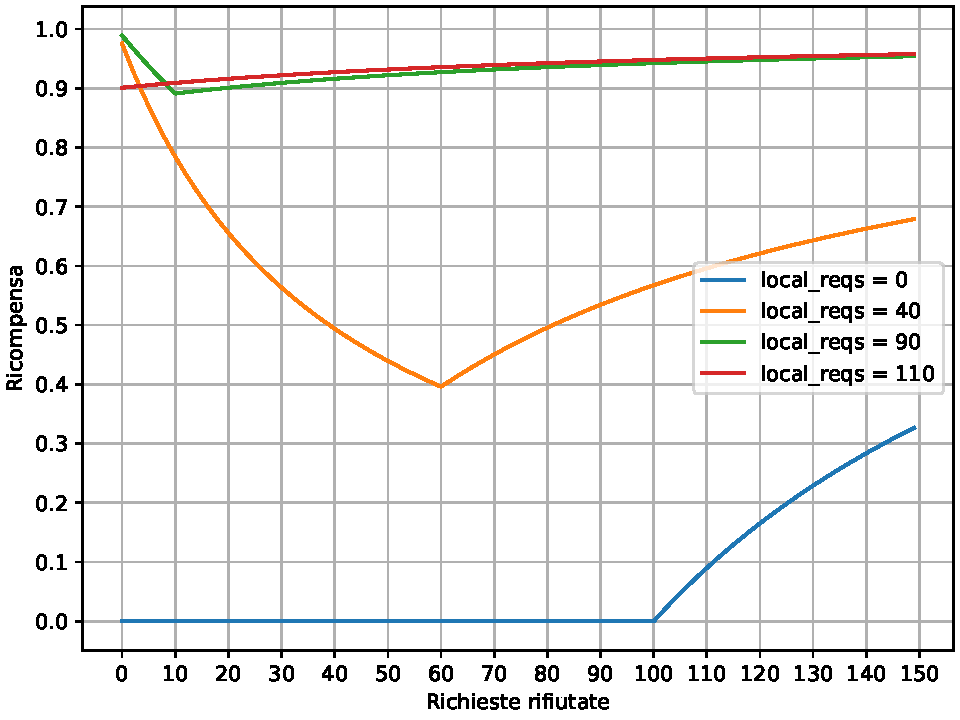
\includegraphics[width=\linewidth]{assets/4/reward_fw_cant_forward.pdf}
        \caption{Con $e^\textnormal{FR} = r^\textnormal{F} = 1$ non è possibile inoltrare richieste, il comportamento è simile alla funzione senza inoltro.}
        \label{fig:4_reward_fw_cant_forward}
    \end{subfigure}

    \begin{subfigure}{.6\textwidth}
        \centering
        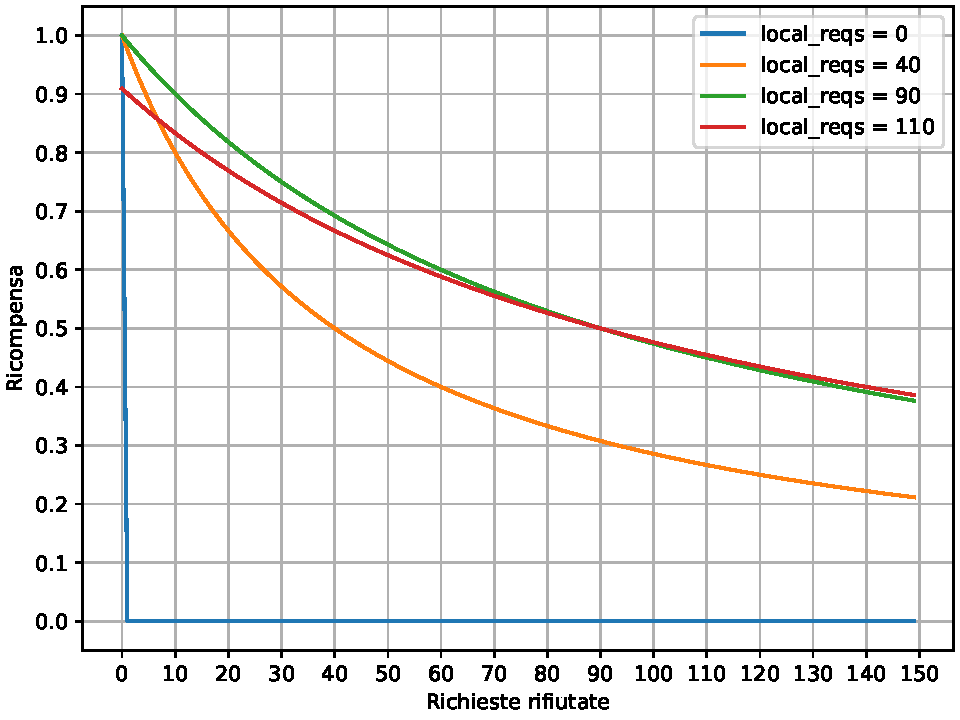
\includegraphics[width=\linewidth]{assets/4/reward_fw_can_forward.pdf}
        \caption{Con $e^\textnormal{FR} = r^\textnormal{F} = 0$ c'è sempre possibilità di inoltrare le richieste.}
        \label{fig:4_reward_fw_can_forward}
    \end{subfigure}

    \begin{subfigure}{.6\textwidth}
        \centering
        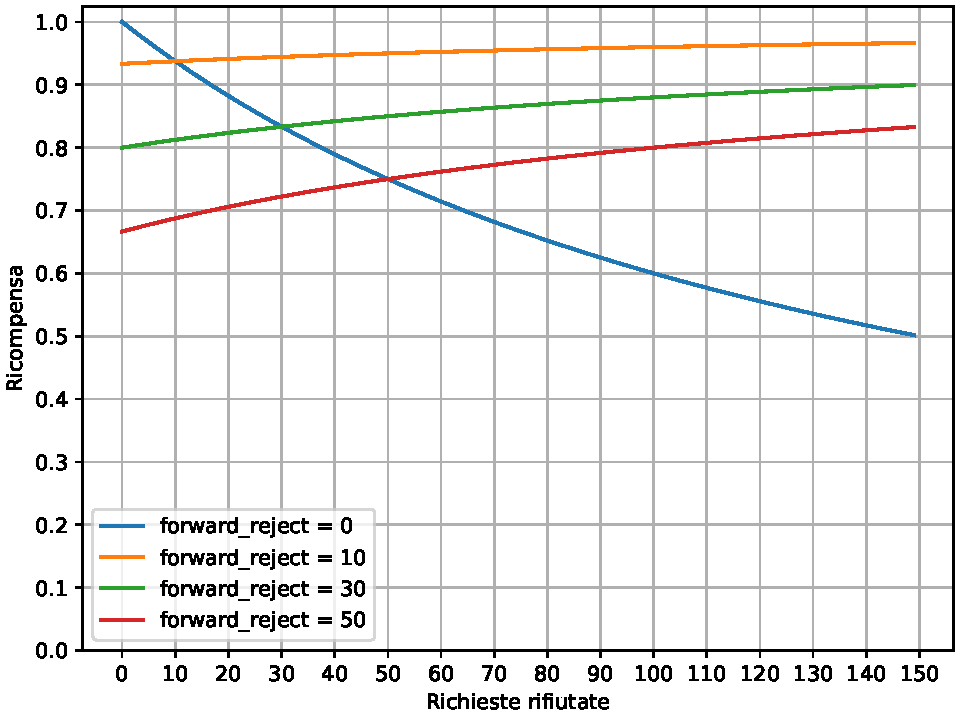
\includegraphics[width=\linewidth]{assets/4/reward_fw_forward_reject.pdf}
        \caption{Effetto del termine $e^\textnormal{FR}$ sulla ricompensa (${r^\textnormal{L} = 100}$, ${r^\textnormal{F} = 50}$).}
        \label{fig:4_reward_fw_forward_reject}
    \end{subfigure}
    
    \caption[Esempi di ricompense per la funzione con inoltro]{Esempi di ricompense per la funzione con inoltro considerando ${q^\textnormal{MAX} = 100}$.}
    \label{fig:4_reward_fw}
\end{figure}

\section{Dinamica degli ambienti}
\label{sec:4_dinamica_ambienti}

\paragraph{Ambienti episodici.} I tre ambienti sono di tipo episodici nonostante lo scenario reale di riferimento sia continuo. Tale scelta è rilevante solo per la sezione sperimentale, poiché agevola la gestione dell'ambiente durante la fasi di addestramento e valutazione; a livello teorico per il problema affrontato separare un ambiente continuo in episodico non perde di generalità.

L'episodio, nel problema affrontato, modella una giornata di 24 ore di distribuzione del carico. Ogni episodio dura esattamente 288 passi, un passo per 5 minuti che coprono l'arco della giornata. La scelta di considerare 5 minuti è motivata dal desiderio di dare tempo agli agenti, nel corrispettivo scenario reale, di reagire con maggiore robustezza ai cambiamenti nel carico su un periodo più esteso dei secondi o del singolo minuto.

\paragraph{Differenze dei tre ambienti.} Le differenze dei tre ambienti si concentrano sullo spazio delle azioni, osservazioni e funzione di ricompensa, poiché sono tre aspetti legati tra di loro. Solo gli ambienti BASE e SYM questi tre aspetti sono omogenei per tutti gli agenti, perché o tutti possono inoltrare o nessuno può; l'ambiente ASYM invece una parte degli agenti possono inoltrare e un'altra no.

Una differenza importante riguarda anche la gestione delle richieste inoltrate in ingresso da altri agenti: in ASYM e SYM le richieste di questo tipo sono elaborate localmente solo dopo aver elaborato le richieste in ingresso dirette per un nodo. In BASE questo meccanismo è assente, poiché nessun agente può inoltrare.

\paragraph{} Il funzionamento dell'ambiente segue le seguenti fasi:

\begin{enumerate}
    \item Inizializzazione: l'ambiente viene inizializzato con i valori di $q^\textnormal{MAX}$ per ogni agente, un contatore per il passo, il generatore di numeri pseudocasuali e la tipologia di carico in ingresso, con la scelta o generazione delle richieste (descritti nella \Cref{sec:5_scenari}).

    \item Azione: ogni agente sceglie un'azione $(p^\textnormal{L}, p^\textnormal{F}, p^\textnormal{R})$ di distribuzione del carico, in base all'osservazione ricevuta. L'ambiente converte i valori percentuali in assoluti sulla base del carico in ingresso per quel passo, ottenendo $(r^\textnormal{L}, r^\textnormal{F}, r^\textnormal{R})$.

    \item Gestione del carico: a partire dal numero di richieste da distribuire, per ogni agente l'ambiente processa le richieste locali occupando gli slot della coda locale. Inoltra le richieste, per gli agenti che sono in grado di inoltrare, e le richieste inoltrare in ingresso occupano gli slot con priorità secondaria rispetto alle richieste locali.

    \item Calcolo della ricompensa: l'ambiente, in base agli effetti dell'azione sullo stato, calcola la ricompensa per ogni agente.

    \item Avanzamento del passo: l'ambiente incrementa il contatore dei passi, svuota la coda locale e genera le nuove osservazioni da restituire agli agenti. Se non è l'ultimo passo, torna alla fase 2. 

    \item Conclusione dell'episodio: essendo l'ambiente episodico, al termine dell'ultimo passo viene restituito un segnale di terminazione all'agente e viene effettuato un ripristino dell'ambiente, tornando alla fase 1.
\end{enumerate}